% *********************** Це є Розділ 1 ************************************

 \markright{\underline {\it Розділ 1. Постановка задачі}}

 \setcounter{chapter}{0}
 \chapter{Постановка задачі штучного інтелекту}

 
 \par У цьому розділі приведено визначення методу Reinforcement Learning (RL), 
 а також розглянуто проблеми, що виникають при його використанні у відеоіграх. 

 \section{Навчання з підкріпленням}
  \setcounter{equation}{0}
 \setcounter{theorem}{0}

 \par Навчання з підкріпленням (RL) - це метод машинного навчання (ML), 
 який навчає модель приймати рішення для досягнення найоптимальніших 
 результатів. Він імітує процес навчання методом спроб і помилок, який
  людина використовує для досягнення своїх цілей. Дії моделі,
  які сприяють досягненню мети, посилюються, тоді як дії,
  які відволікають - ігноруються.
  \newpage
 \parАлгоритми RL використовують парадигму заохочення і покарання для обробки даних,
  навчаючись на основі зворотного зв'язку від кожної дії. Вони самостійно знаходять найкращі 
  шляхи для досягнення кінцевого результату, іноді включаючи короткострокові жертви. RL допомагає
   системам штучного інтелекту досягати оптимальних результатів у непередбачуваних умовах.

 Проблеми RL можна уявити як систему з агента і середовища. Середовище має стан, який агент 
 спостерігає для вибору дії. Обрана дія виконується, середовище переходить у новий стан, і агент
  отримує винагороду. Цикл "стан $\rightarrow$ дія $\rightarrow$ винагорода" повторюється до завершення середовища, наприклад,
   до вирішення проблеми. Цей процес відбувається протягом епізоду.
\begin{figure}[h]
  \centering
  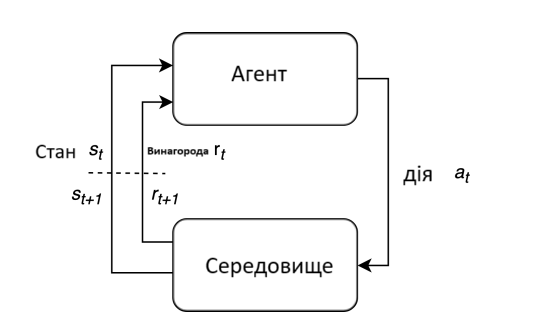
\includegraphics[scale=1]{Pictures/RL_Diagram.png}
  \caption{Діаграма управління}
  \label{fig:RLloopdiagram}
\end{figure}
\newpage
Функція, що породжує дії агента, називається {\em політикою(policy)}. Формально, 
політика - це функція, яка деякому стану співставляє дію.

\section{Проблеми Ігрового середовища}
  \setcounter{equation}{0}
 \setcounter{theorem}{0}

 У нас є комп'ютерна відеогра, в якій агент має навчитися приймати оптимальні рішення для досягнення заданих цілей, таких як перемога над суперниками або виконання місій. Метою є розробити методи, що дозволяють агенту, використовуючи алгоритми глибокого навчання з підкріпленням (DRL), ефективно навчатися та адаптуватися до складного і динаміч\-ного ігрового середовища.

 Основні виклики, з якими ми стикаємося:
 
 \begin{itemize}
   \item \emph{Візуальне сприйняття:} Агент повинен аналізувати візуальні дані з екрану гри та перетворювати їх у числові значення, придатні для алгоритмів навчання.
   \item \emph{Високорозмірний простір станів:} Ігрове середовище характеризується складним і високорозмірним простором станів, що ускладнює ефективне представлення та обробку інформації.
   \item \emph{Великий простір дій:} Агент має широкий набір можливих дій, які потрібно оптимально використовувати для досягнення цілей гри.
   \item \emph{Нагороди:} Нагороди в грі можуть бути рідкісними та відкладеними, що ускладнює процес навчання агента.
 \end{itemize}